\section{Benchmarks de l'approche génétique}

Il s'agira dans cette partie d'évaluer le temps que met notre approche génétique en fonction des paramètres d'entrée. Il peut en effet être intéressant de savoir si notre algorithme évolue de façon linéaire ou exponentielle par rapport à ces derniers.

Le fichier de données considéré correspond au \textit{Barnes - setb4c9}. En effet, il comporte $15$ jobs et $11$ machines ce qui le rend intéressant de par la taille du problème.

Le code servant à réaliser les benchmarks est disponible dans le fichier \textit{benchmarks.py}.

\subsection{Comparaison du temps d'exécution par rapport à la taille de la population}

La génération maximale est ici fixée à $100$. Nous faisons évoluer la taille de la population de façon logarithmique entre $1$ et $10000$.

\begin{figure}[!h]
    \centering
    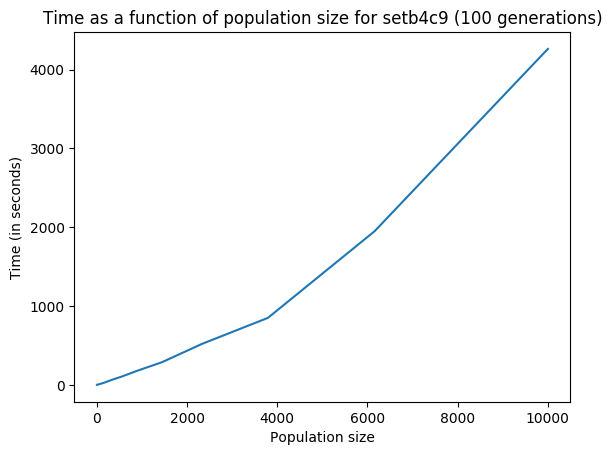
\includegraphics[]{report/Pictures/setb4c9_benchmarks_population.png}
\end{figure}

A $max\_generation$ fixé, le temps de calcul n'est pas linéaire en fonction du nombre d'individus dans la population. Il est intéressant de savoir s'il est polynomial ou exponentiel.

Afin d'obtenir de meilleurs résultats, on commence par faire une interpolation par spline de notre ensemble de points. Une spline est une fonction polynomiale par morceaux et ce type d'interpolation locale est plus efficace qu'une interpolation globale. Nous ne rentrerons pas plus dans les détails de ce qu'est une spline, la littérature sur internet étant très complète à ce sujet. Cette spline permettra de densifier notre ensemble de points de façon artificielle et sera utile pour calculer des résidus.

\begin{figure}[!h]
    \centering
    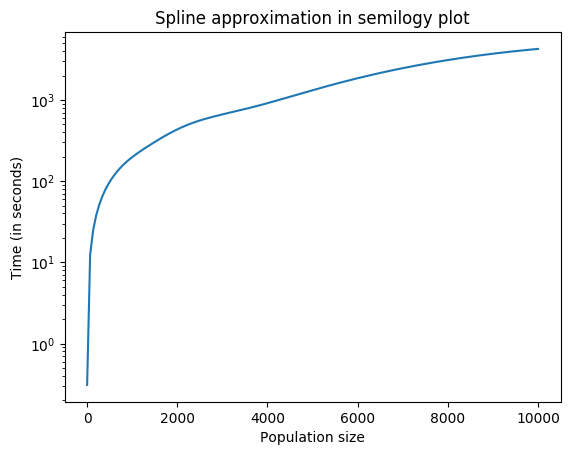
\includegraphics[]{report/Pictures/setb4c9_expo_semilogy.png}
\end{figure}

En utilisant une échelle logarithmique pour les ordonnées, on peut déjà éliminer l'hypothèse d'une complexité temporelle exponentielle. En effet, dans un tel repère, les représentations graphiques des fonctions exponentielles sont des droites.

Maintenant que ce point est réglé, évaluons différentes interpolations polynomiales.

\begin{figure}[!h]
    \centering
    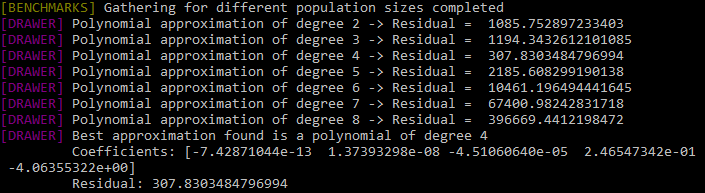
\includegraphics[width=\linewidth]{report/Pictures/setb4c9_approximation_result.png}
\end{figure}

Soit \textit{xdata} la liste des tailles de population évaluées par l'algorithme de benchmarks. On commence par construire une liste de 150 points compris entre $xdata[0]$ et $xdata[-1]$, autrement dit la première et la dernière valeur de la liste \textit{xdata}.

\begin{lstlisting}
x = np.linspace(xdata[0], xdata[-1], 150)
\end{lstlisting}

On évalue ainsi le résidu pour des polynômes de degrés différents, ici entre 2 et 8. Le résidu correspond à la somme des norme 2 de la différence entre notre approximation polynomiale et les valeurs de la spline :

$$ r_i = \sum_{j = 1}^{150} \left\| s(x_j) - p_i(x__j) \right\| $$

Ici, $r_i$ correspond au résidu du polynôme de degré $i$, $s$ correspond à notre spline et $p_i$ à la fonction polynomiale de degré $i$ obtenue de la façon suivante :

\begin{lstlisting}
# Find a polynomial to fit the spline
coefficients = np.polyfit(xdata, ydata, i)
p_i = np.poly1d(coefficients)
\end{lstlisting}

Nous avons fait le choix de construire l'interpolation polynomiale en se basant uniquement sur les points calculés par l'algorithme de benchmarks et non sur la spline. Les calculs sont plus rapides car il y a moins de points et la perte de précision dans le calcul des coefficients est négligeable, ces derniers nous intéressant peu.

Le résidu le plus faible est obtenu pour un polynôme de degré 4, notre complexité temporelle en fonction de la taille de la population est donc en $\mathcal{O}(n^4)$.

\begin{figure}[!h]
    \centering
    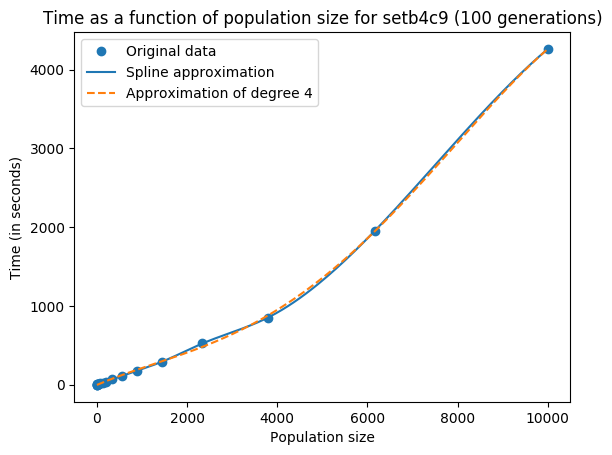
\includegraphics[]{report/Pictures/setb4c9_benchmarks_population_approximated.png}
\end{figure}

\subsection{Comparaison du temps d'exécution par rapport à la génération maximale}

La taille de la population est ici fixée à $100$. Nous faisons évoluer la génération maximale de façon logarithmique entre $1$ et $10000$.

\begin{figure}[!h]
    \centering
    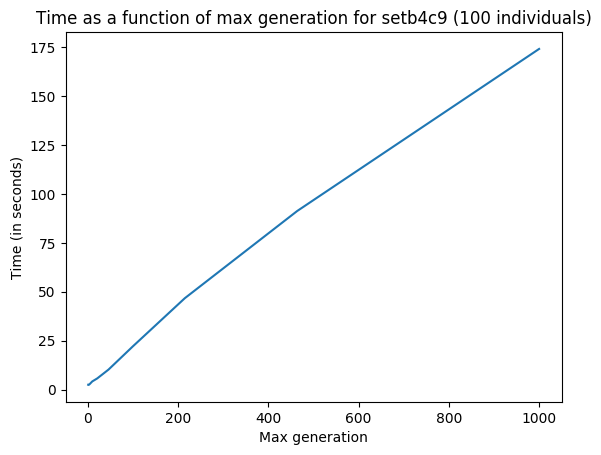
\includegraphics[]{report/Pictures/setb4c9_benchmarks_generation.png}
\end{figure}

A $population\_size$ fixé, le temps de calcul est linéaire en fonction de la génération maximale. Ce résultat n'est pas surprenant, mais il nous semblait important de le vérifier.

\newpage

\subsection{Comparaison du temps d'exécution par rapport à la taille de la population et la génération maximale}

\begin{figure}[!h]
    \centering
    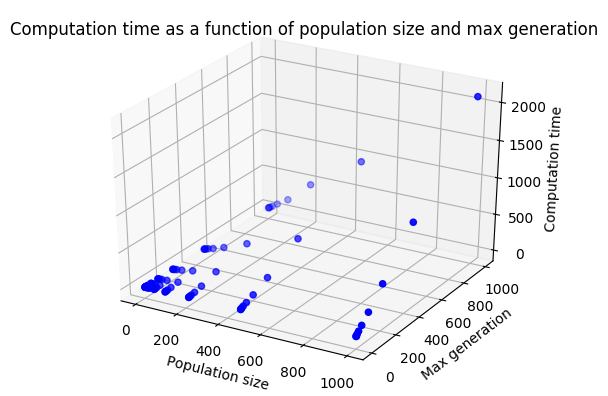
\includegraphics[]{report/Pictures/setb4c9_benchmarks_generation_with_computation_time.png}
\end{figure}

On retrouve bien le côté linéaire par rapport à la génération maximale et polynomial par rapport à la taille de la population.

\newpage

\subsection{Comparaison de la fonction objective par rapport à la taille de la population et la génération maximale}

\begin{figure}[!h]
    \centering
    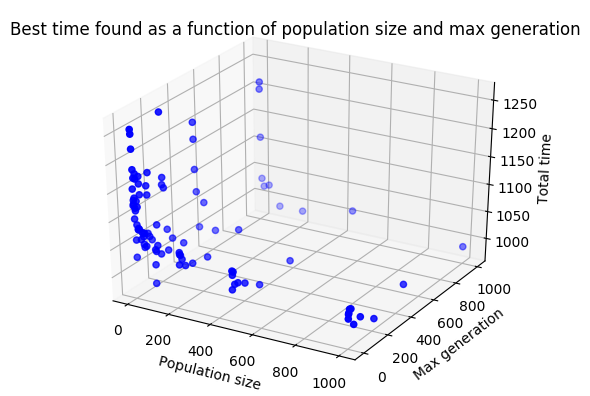
\includegraphics[]{report/Pictures/setb4c9_benchmarks_generation_with_solution_time.png}
\end{figure}

Nous avons également décidé de regarder le temps de la solution renvoyé par l'algorithme génétique en fonction de la taille de la population et de la génération maximale.

Sur des tailles de populations petites, la solution renvoyée s'améliore très rapidement et fortement. Par contre, ces évolutions sont moins distinguables pour des tailles de populations importantes.

\newpage